% RRINT
%
The data for register access-use intervals are
shown in Figures \ref{fig:aa_rrint} 
and \ref{fig:ab_rrint}.
Results from benchmark programs BZIP2, COMPRESS, CRAFTY, GCC, and GO
are shown in Figure \ref{fig:aa_rrint} while the results
from programs GZIP, IJPEG, MCF, PARSER, and VORTEX are shown in
Figure \ref{fig:ab_rrint}.
%
\begin{figure}
\centering
\epsfig{file=aa_rrint.eps,width=6.0in}
\caption{{\em Register Access-Use Intervals.} 
Data results for the 
BZIP2, COMPRESS, CRAFTY, GCC, and GO programs are shown.
The density is shown on the left and the distribution is shown
on the right.
All intervals are measured in dynamic numbers of executed instructions.}
\label{fig:aa_rrint}
\end{figure}
%
\begin{figure}
\centering
\epsfig{file=ab_rrint.eps,width=6.0in}
\caption{{\em Register Access-Use Intervals.} 
Data results for the
GZIP, IJPEG, MCF, PARSER, and VORTEX programs are shown.
The density is shown on the left and the distribution is shown
on the right.
All intervals are measured in dynamic numbers of executed instructions.}
\label{fig:ab_rrint}
\end{figure}
%
%
% RLIFE

The data for register def-last-use (or useful-lifetime) intervals are
shown in Figures \ref{fig:aa_rlife} 
and \ref{fig:ab_rlife}.
%
\begin{figure}
\centering
\epsfig{file=aa_rlife.eps,width=6.0in}
\caption{{\em Register Def-Last-Use Intervals.} 
Data results for the 
BZIP2, COMPRESS, CRAFTY, GCC, and GO programs are shown.
The density is shown on the left and the distribution is shown
on the right.
All intervals are measured in dynamic numbers of executed instructions.}
\label{fig:aa_rlife}
\end{figure}
%
\begin{figure}
\centering
\epsfig{file=ab_rlife.eps,width=6.0in}
\caption{{\em Register Def-Last-Use Intervals.} 
Data results for the
GZIP, IJPEG, MCF, PARSER, and VORTEX programs are shown.
The density is shown on the left and the distribution is shown
on the right.
All intervals are measured in dynamic numbers of executed instructions.}
\label{fig:ab_rlife}
\end{figure}
%
%
% RUSE

The data for register def-use intervals are
shown in Figures \ref{fig:aa_ruse} 
and \ref{fig:ab_ruse}.
%
\begin{figure}
\centering
\epsfig{file=aa_ruse.eps,width=6.0in}
\caption{{\em Register Def-Use Intervals.} 
Data results for the 
BZIP2, COMPRESS, CRAFTY, GCC, and GO programs are shown.
The density is shown on the left and the distribution is shown
on the right.
All intervals are measured in dynamic numbers of executed instructions.}
\label{fig:aa_ruse}
\end{figure}
%
\begin{figure}
\centering
\epsfig{file=ab_ruse.eps,width=6.0in}
\caption{{\em Register Def-Use Intervals.} 
Data results for the
GZIP, IJPEG, MCF, PARSER, and VORTEX programs are shown.
The density is shown on the left and the distribution is shown
on the right.
All intervals are measured in dynamic numbers of executed instructions.}
\label{fig:ab_ruse}
\end{figure}
%
%
